\documentclass[tikz,border=20pt]{standalone}
\usetikzlibrary{calc,arrows.meta,decorations.markings}
\usepackage{amsmath,amssymb}

\begin{document}
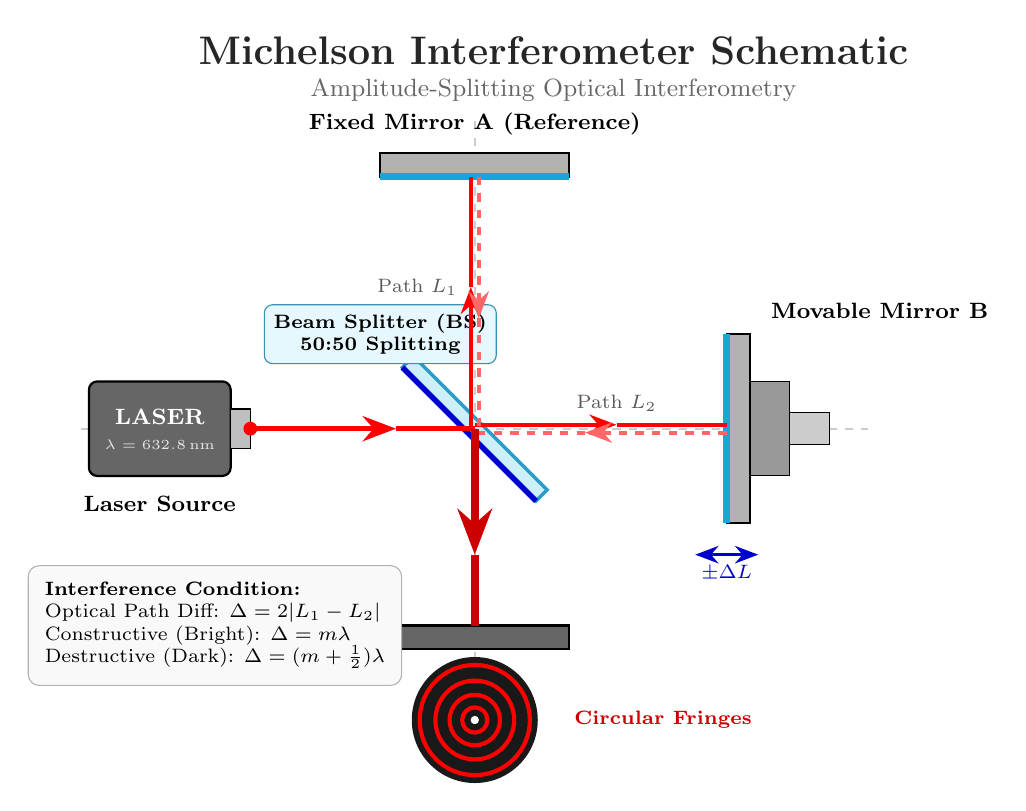
\begin{tikzpicture}[x=1cm, y=1cm, >=Stealth]

  % Title
  \node[font=\bfseries\Large, text=black!85] at (3.5, 4.8) {Michelson Interferometer Schematic};
  \node[font=\small, text=gray!80!black] at (3.5, 4.3) {Amplitude-Splitting Optical Interferometry};

  % Optical Axis Guidelines
  \draw[gray!40, dashed, line width=0.8pt] (-2.5, 0) -- (7.5, 0);
  \draw[gray!40, dashed, line width=0.8pt] (2.5, -4.0) -- (2.5, 4.0);

  % 1. LASER SOURCE (Left: -1.5, 0)
  \filldraw[fill=gray!80!black, draw=black, thick, rounded corners=3pt] (-2.4, -0.6) rectangle (-0.6, 0.6);
  \filldraw[fill=gray!50, draw=black] (-0.6, -0.25) rectangle (-0.35, 0.25);
  \fill[red] (-0.35, 0) circle (2.5pt);
  \node[font=\bfseries\footnotesize, text=white] at (-1.5, 0.15) {LASER};
  \node[font=\tiny, text=gray!20] at (-1.5, -0.2) {$\lambda = 632.8\,\text{nm}$};
  \node[font=\bfseries\footnotesize, below=4pt] at (-1.5, -0.6) {Laser Source};

  % 2. BEAM SPLITTER (Center: 2.5, 0, rotated 45 deg)
  \begin{scope}[shift={(2.5, 0)}, rotate=45]
    \filldraw[fill=cyan!20, draw=cyan!80!black, line width=1.2pt] (-0.1, -1.2) rectangle (0.1, 1.2);
    \draw[blue!80!black, line width=2pt] (-0.1, -1.2) -- (-0.1, 1.2);
  \end{scope}
  \node[draw=cyan!70!black, fill=cyan!10, rounded corners=3pt, font=\bfseries\scriptsize, align=center] at (1.3, 1.2) {
    Beam Splitter (BS)\\50:50 Splitting
  };

  % 3. REFERENCE MIRROR A (Top: 2.5, 3.2)
  \filldraw[fill=gray!60, draw=black, thick] (1.3, 3.2) rectangle (3.7, 3.5);
  \draw[cyan!90!black, line width=2.5pt] (1.3, 3.2) -- (3.7, 3.2);
  \node[font=\bfseries\footnotesize, above=3pt] at (2.5, 3.5) {Fixed Mirror A (Reference)};
  \node[font=\scriptsize, text=gray!70!black, left] at (2.4, 1.8) {Path $L_1$};

  % 4. MOVABLE MIRROR B (Right: 5.7, 0)
  \filldraw[fill=gray!60, draw=black, thick] (5.7, -1.2) rectangle (6.0, 1.2);
  \draw[cyan!90!black, line width=2.5pt] (5.7, -1.2) -- (5.7, 1.2);
  \filldraw[fill=gray!80, draw=black] (6.0, -0.6) rectangle (6.5, 0.6);
  % Micrometer screw
  \filldraw[fill=gray!40, draw=black] (6.5, -0.2) rectangle (7.0, 0.2);
  \draw[<->, line width=1.2pt, blue!80!black] (5.3, -1.6) -- (6.1, -1.6) node[midway, below, font=\scriptsize\bfseries] {$\pm\Delta L$};
  \node[font=\bfseries\footnotesize, right=4pt] at (6.0, 1.5) {Movable Mirror B};
  \node[font=\scriptsize, text=gray!70!black, above] at (4.3, 0.1) {Path $L_2$};

  % 5. OBSERVATION SCREEN & DETECTOR (Bottom: 2.5, -2.8)
  \filldraw[fill=gray!80!black, draw=black, thick] (1.3, -2.8) rectangle (3.7, -2.5);
  % Concentric interference rings
  \begin{scope}[shift={(2.5, -3.7)}]
    \fill[black!90] (0, 0) circle (0.8);
    \foreach \r in {0.7, 0.5, 0.32, 0.16} {
      \draw[red, line width=1.5pt] (0, 0) circle (\r);
    }
    \fill[white] (0,0) circle (1.5pt);
  \end{scope}
  \node[font=\bfseries\footnotesize, left=4pt] at (1.3, -2.65) {Screen / Detector};
  \node[font=\scriptsize\bfseries, text=red!80!black, right=4pt] at (3.5, -3.7) {Circular Fringes};

  % 6. LIGHT BEAMS & DIRECTIONAL ARROWS
  % Incident: Laser -> BS
  \draw[red, line width=2pt, ->] (-0.35, 0) -- (1.5, 0);
  \draw[red, line width=2pt] (1.5, 0) -- (2.5, 0);

  % Transmitted: BS -> Mirror B (outgoing)
  \draw[red, line width=1.5pt, ->] (2.5, 0.05) -- (4.3, 0.05);
  \draw[red, line width=1.5pt] (4.3, 0.05) -- (5.7, 0.05);
  % Returning: Mirror B -> BS
  \draw[red!60, dashed, line width=1.5pt, ->] (5.7, -0.05) -- (3.9, -0.05);
  \draw[red!60, dashed, line width=1.5pt] (3.9, -0.05) -- (2.5, -0.05);

  % Reflected: BS -> Mirror A (outgoing)
  \draw[red, line width=1.5pt, ->] (2.45, 0) -- (2.45, 1.8);
  \draw[red, line width=1.5pt] (2.45, 1.8) -- (2.45, 3.2);
  % Returning: Mirror A -> BS
  \draw[red!60, dashed, line width=1.5pt, ->] (2.55, 3.2) -- (2.55, 1.4);
  \draw[red!60, dashed, line width=1.5pt] (2.55, 1.4) -- (2.55, 0);

  % Combined Superposed Beam: BS -> Screen
  \draw[red!80!black, line width=3pt, ->] (2.5, 0) -- (2.5, -1.6);
  \draw[red!80!black, line width=3pt] (2.5, -1.6) -- (2.5, -2.5);

  % 7. FORMULA BOX
  \node[draw=gray!60, fill=gray!5, rounded corners=4pt, font=\scriptsize, align=left, inner sep=6pt] at (-0.8, -2.5) {
    \textbf{Interference Condition:}\\
    Optical Path Diff: $\Delta = 2|L_1 - L_2|$\\
    Constructive (Bright): $\Delta = m\lambda$\\
    Destructive (Dark): $\Delta = (m + \frac{1}{2})\lambda$
  };

\end{tikzpicture}
\end{document}
